\problemname{Tower}
There are many legends concerning the Leaning Tower of Toruń.
The wall of the tower is a circle with $N\geq 3$ evenly spaced doors (in other
words, the doors are the vertices of a regular $N$-gon). The doors are numbered
from $0$ to $N-1$, but in a \textbf{random order}.
Please refer to the scoring section for more details about this.

One of the less known legends describes how every new inhabitant of
the tower had to complete a certain challenge. The goal of the challenge
was to list the doors, starting with some door and then walking around the circle
(clockwise or counterclockwise), visiting each door exactly once.

This needs to be done without actually seeing the tower.
Instead, the new inhabitant can ask questions of the following form:
``Given three distinct doors $x,y,z$, which pairs of doors are the closest to each other: $\{x,y\}$,
$\{y,z\}$, or $\{z,x\}$?''. The answer to such a question are all pairs (among $\{x,y\}$, $\{y,z\}$ and $\{z,x\}$)
of doors with the smallest Euclidean distance. The distance is simply the length of the shortest
segment connecting the doors.
Your task is to write a program that will ask a small number of such questions
to determine the order of the doors.

\section*{Interaction}
This is an interactive task. You should write a program which finds a correct
solution to the task and communicates with the interactor by reading from
the standard input and writing to the standard output.

At the beginning of the interaction, your program should read two integers
$t$ and $k$ $(1 \leq t \leq 100$, $1\leq k\leq 12\,000$) from the standard input,
denoting the number of test cases and the maximum allowed average number of queries,
respectively. See the scoring section for more information about the latter.

For each test case, your program should first read a single integer $n$ $(3 \leq n \leq 500)$
from the standard input, denoting the number of doors in the tower.

Then your program should ask the questions in the following way:
\begin{itemize}
\item Your program should write a single line in the form of\vspace{3mm}\\
\texttt{? $x$ $y$ $z$} \vspace{3mm}\\
to the standard output, where $x$, $y$, and $z$ are distinct
integers ($0\leq x,y,z\leq n-1$). This line represents a single question
concerning doors $x$, $y$, and $z$.

\item The response will be given as:\vspace{3mm}\\
\texttt{$r$\\
$a_1$ $b_1$\\
$\ldots$\\
$a_r$ $b_r$}\vspace{3mm}\\
where $r$ is an integer ($1\leq r\leq 3$)  representing the number of
pairs of doors with the smallest distance.
Each such pair is described by two integers $a_{i}$ and $b_{i}$ ($a_{i}, b_{i} \in \{x,y,z \}$ and $a_{i} < b_{i}$).
\end{itemize}

\noindent Once you have determined the order of the doors, you should write a single line
in the form of\vspace{3mm} \\
\texttt{! $x_0$ $x_1$ $\ldots$ $x_{n-1}$}\vspace{3mm}\\
to the standard output, where $x_0, x_1, \ldots, x_{n-1}$ is the order of the doors
as described in the task statement.
Please note that there are exactly $2n$ possible
correct answers since you can output the order starting from any door and then going in either direction.
Any of them will be accepted.

\textbf{Keep in mind that after each query or answer you have to flush the output buffer using
\texttt{cout.flush()} (or \texttt{fflush(stdout)} if using \texttt{printf}) in C++
or \texttt{sys.stdout.flush()} in Python.} Otherwise your program may
receive a \texttt{Time Limit Exceeded} verdict.

After writing the answer to the interactor, your program should immediately proceed to the next test case
or end the interaction if all test cases have been processed.

Your program cannot open any files or use any other resources. It can use the standard
error stream for debugging purposes, but please mind that writing to this
stream takes time.

Please also note that the interactor is not adaptive, meaning that the initial order of the doors
is fixed beforehand in each test case and does not change during the interaction.

\section*{Example interaction}
Suppose we have only one test case with $n=6$, and the order of the doors is $5, 3, 0, 2, 1, 4$.
The interaction could look as follows:

\begin{center}
\begin{tabular}{|l|l|l|}
\hline
\textbf{Interactor} & \textbf{Your program} & \textbf{Comment} \\
\hline
\texttt{1 100} & & $t=1$ and $k=100$. \\ \hline
\texttt{6} & & Interactor gives the number of doors in the first test case. \\ \hline
& \texttt{? 0 1 2} & Your program asks which pairs of doors are the closest. \\ \hline
\shortstack{\texttt{2} \\ \texttt{0 2} \\ \texttt{1 2}} & & Pairs of doors $\{0,2\}$ and $\{1,2\}$ are the closest. \\ \hline
& \texttt{? 4 1 3} & Your program asks which pairs of doors are the closest. \\ \hline
\shortstack{\texttt{1} \\ \texttt{1 4}} & & Pair $\{1,4\}$ is the closest. \\ \hline
& \texttt{? 0 5 1} & Your program asks which pairs of doors are the closest. \\ \hline
\shortstack{\texttt{3} \\ \texttt{0 5} \\ \texttt{0 1} \\ \texttt{1 5}} & & Pairs $\{0,5\}$, $\{0,1\}$, and $\{1,5\}$ are the closest. \\ \hline
& \texttt{! 4 5 3 0 2 1} & Your program correctly outputs the order of the doors. \\ \hline
\end{tabular}
\end{center}


\medskip

\begin{center}
\begin{figure}[h!]
    \centering
    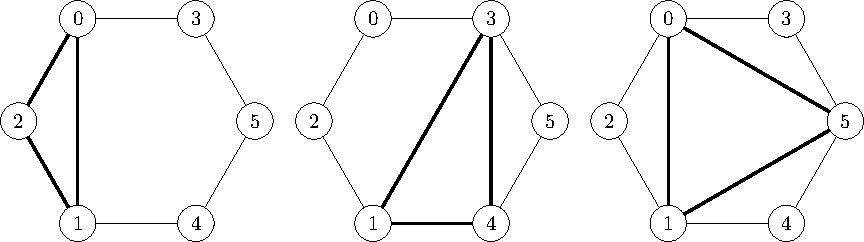
\includegraphics[width=1\textwidth]{example.pdf}
\end{figure}
\end{center}

\medskip

\section*{Explanation of above sample}
The pictures above show the doors with their numbers along the walls of the tower.
In the first picture from the left
a triangle formed by the doors with numbers $0, 1, 2$ is shown, corresponding to the first query of
your program. We can see that the pairs
$\{0,2\}$ and $\{1,2\}$ are the closest. In the middle picture a triangle formed by the doors with numbers
$1, 4, 3$ is shown, corresponding to the second query of your program.
We can clearly see that the pair $\{1,4\}$ is the closest. In the third picture from the left
a triangle formed by the doors with numbers $0, 1, 5$ is shown, corresponding to the third query
of your program. We can clearly see that all the pairs of doors
are equally close to each other.

Please note that the sequences $0,2,1,4,5,3$ or $5,4,1,2,0,3$ (and a couple others)
would also be correct answers in this case.

\section*{Scoring}

Scoring for this problem is divided into subtasks. For each subtask there is exactly one test
and this single test contains exactly $t=100$ test cases.
For each test, the average number of queries asked by your program is calculated by taking the total number of queries
among all test cases and dividing it by the number of test cases. If this average is greater than $k$ for a given subtask,
you will receive a score of $0$ for that subtask. Otherwise, for subtasks 1 to 4, you will receive full score for that subtask.

For the last subtask, your score will be calculated as follows.
Let $k^{*}$ be the actual average number of queries asked by your program. Then, the
number of points is given by the following formula:
\[
\left\lceil 56 \cdot \min\left(1, \frac{12000-k^{*}}{7800}\right)\right\rceil,
\]
meaning that your score increases linearly from $0$ to $56$ as $k^{*}$ goes from $12000$ to $4200$.

Please note that if your program gives an incorrect answer to any test case, you will receive a score
of $0$ for that subtask
regardless of the number of queries asked.

The additional constraints for each subtask are in the table below.

\begin{center}
\begin{tabular}{|c|p{13cm}|c|}
\hline
\textbf{Subtask} & \textbf{Constraints} & \textbf{Points} \\ \hline
1 & $k=8000, 3\leq n\leq 9$ & 6 \\ \hline
2 & $k=4500, 40\leq n\leq 50$ & 7 \\ \hline
3 & $k=3000, 90\leq n\leq 100$ & 9 \\ \hline
4 & $k=4500, n=400$, there is a correct answer $x_0,\dots,x_{n-1}$ where $x_i=i$ for $200\leq i\leq 399$ & 22 \\ \hline
5 & $k=12\,000, n=500$ & up to 56 \\ \hline
\end{tabular}
\end{center}

Moreover, you can assume that each test case has been generated by first choosing
$n$ \textbf{uniformly at random} from all values of $n$ satisfying the constraints of a given subtask,
and then choosing the order of the doors \textbf{uniformly at random} from all orders
of $n$ doors satisfying the constraints of a given subtask.
